\section{Performance evaluation}\label{sec:evaluation}

We evaluate the computational cost of DSphinx and its destination-bound credential mechanism across three stages: system setup, credential issuance, and packet construction and processing. 
Our experiments examine sensitivity to the reconstruction threshold $t$ and the path length $\ell$, distinguishing setup and issuance costs from recurring per-packet computation.

\subsection{Implementation and experimental setup}

We implement a Python prototype\footnote{\artifact} using \texttt{mclbn256} library for DSphinx and its credential protocol.
The zero-knowledge component uses Groth16 through \texttt{snarkjs}, with circuits compiled using Circom. 
Elliptic-curve operations within the circuit use Baby Jubjub.

All measurements report CPU time and were obtained on a laptop with a 13th-generation Intel Core i7-13700HX processor running at $3.70\,\mathrm{GHz}$. 
The prototype executes a multithreaded simulation on a single machine, with 20 mixnodes, 50 authorities, and 10 clients. 
Each client requests a credential for its own address and subsequently sends 10 packets to that address over randomly sampled routes, yielding 100 packets per run.\todo[]{Run more iterations of each run to smooth curves}
Figures report mean CPU times for the corresponding operations and parameter settings. 
These component measurements do not establish end-to-end network latency or system throughput.

For the fixed blacklist of five addresses used in our experiments, circuit compilation takes approximately $150 \mathrm{ms}$ and produces $5 375$ constraints.\todo[]{Reverify this value}
The circuit fits within a Powers of Tau setup with exponent 13, corresponding to a capacity of $2^{13}=8 192$ constraints. 
Circuit compilation is performed once for this blacklist configuration.

\paragraph{Prototype limitation.}
Credential issuance requires a proof of the relation $\blind{\Delta}=r\Delta$, where $\Delta$ encodes the destination $d$ on the BN256 curve used in the packet header. 
However, the Baby Jubjub arithmetic used by our Circom circuit cannot directly express this relation over BN256. 
Addressing this mismatch requires either implementing non-native BN256 arithmetic within the circuit, blowing up circuit complexity, or selecting compatible curves between the header encoding and the proof system.
We leave this integration to future work.

For benchmarking, we therefore use an intermediate approach.
The client encodes the destination on both curves and includes both representations in its credential request. 
The authority verifies the proof using the Baby Jubjub representation and, if verification succeeds, signs the BN256 representation.

This approach is used exclusively for performance evaluation.
The proof does not establish that the two representations correspond to the same destination, making the workaround unsuitable for deployment. 
In our experiments, both representations are generated from the same destination by construction, allowing the remaining protocol operations to be executed without modification. 
The measurements therefore capture these operations, but exclude the cost of enforcing consistency between the two representations. 
Replacing this workaround with a compatible curve configuration is a necessary step toward a complete implementation.

\subsection{System setup}

System setup comprises a Distributed Key Generation (DKG), a Powers of Tau ceremony (PoT), and circuit-specific Groth16 setup togenerate the Common Reference String (CRS). 
Issued credentials remains valid as long as $\PSI_2$ is valid.
Therefore, an epoch-based deployment can repeat DKG to rotate $\PSI_1$ and $\PSI_2$, and require clients to obtain credentials for the new epoch.
The Powers of Tau ceremony is generated once but new contribution can be added.
The CRS need to be rerun after circuit modification (i.e. changing the hardcoded blacklist) or when new contributions are added to the PoT.

Let $c$ denote the number of setup contributions. 
This parameter is independent of the reconstruction threshold $t$.
However, we have decided to fix $c=t$ in the setup experiments. 
For the evaluated circuit, the measured trends are approximately:
\begin{align*}
    T_{\mathrm{PoT}}(c) &\approx (25 + 2c)\,\mathrm{s},\\
    T_{\mathrm{CRS}}(c) &\approx (6 + \frac{3}{5}c)\,\mathrm{s}.
\end{align*}

As shown in Figure~\ref{im:setup_time}, DKG accounts for a comparatively small fraction ($\le 0.5 \mathrm{s}$)\todo[]{Verify this value} of setup computation across the tested thresholds. 
The total setup cost ranges from approximately $40\,\mathrm{s}$ to $160\,\mathrm{s}$, reaching the latter value at $t=50$. 
Thus, setup is dominated by the zero-knowledge part, mainly the PoT. 
\begin{figure}
    \centering
    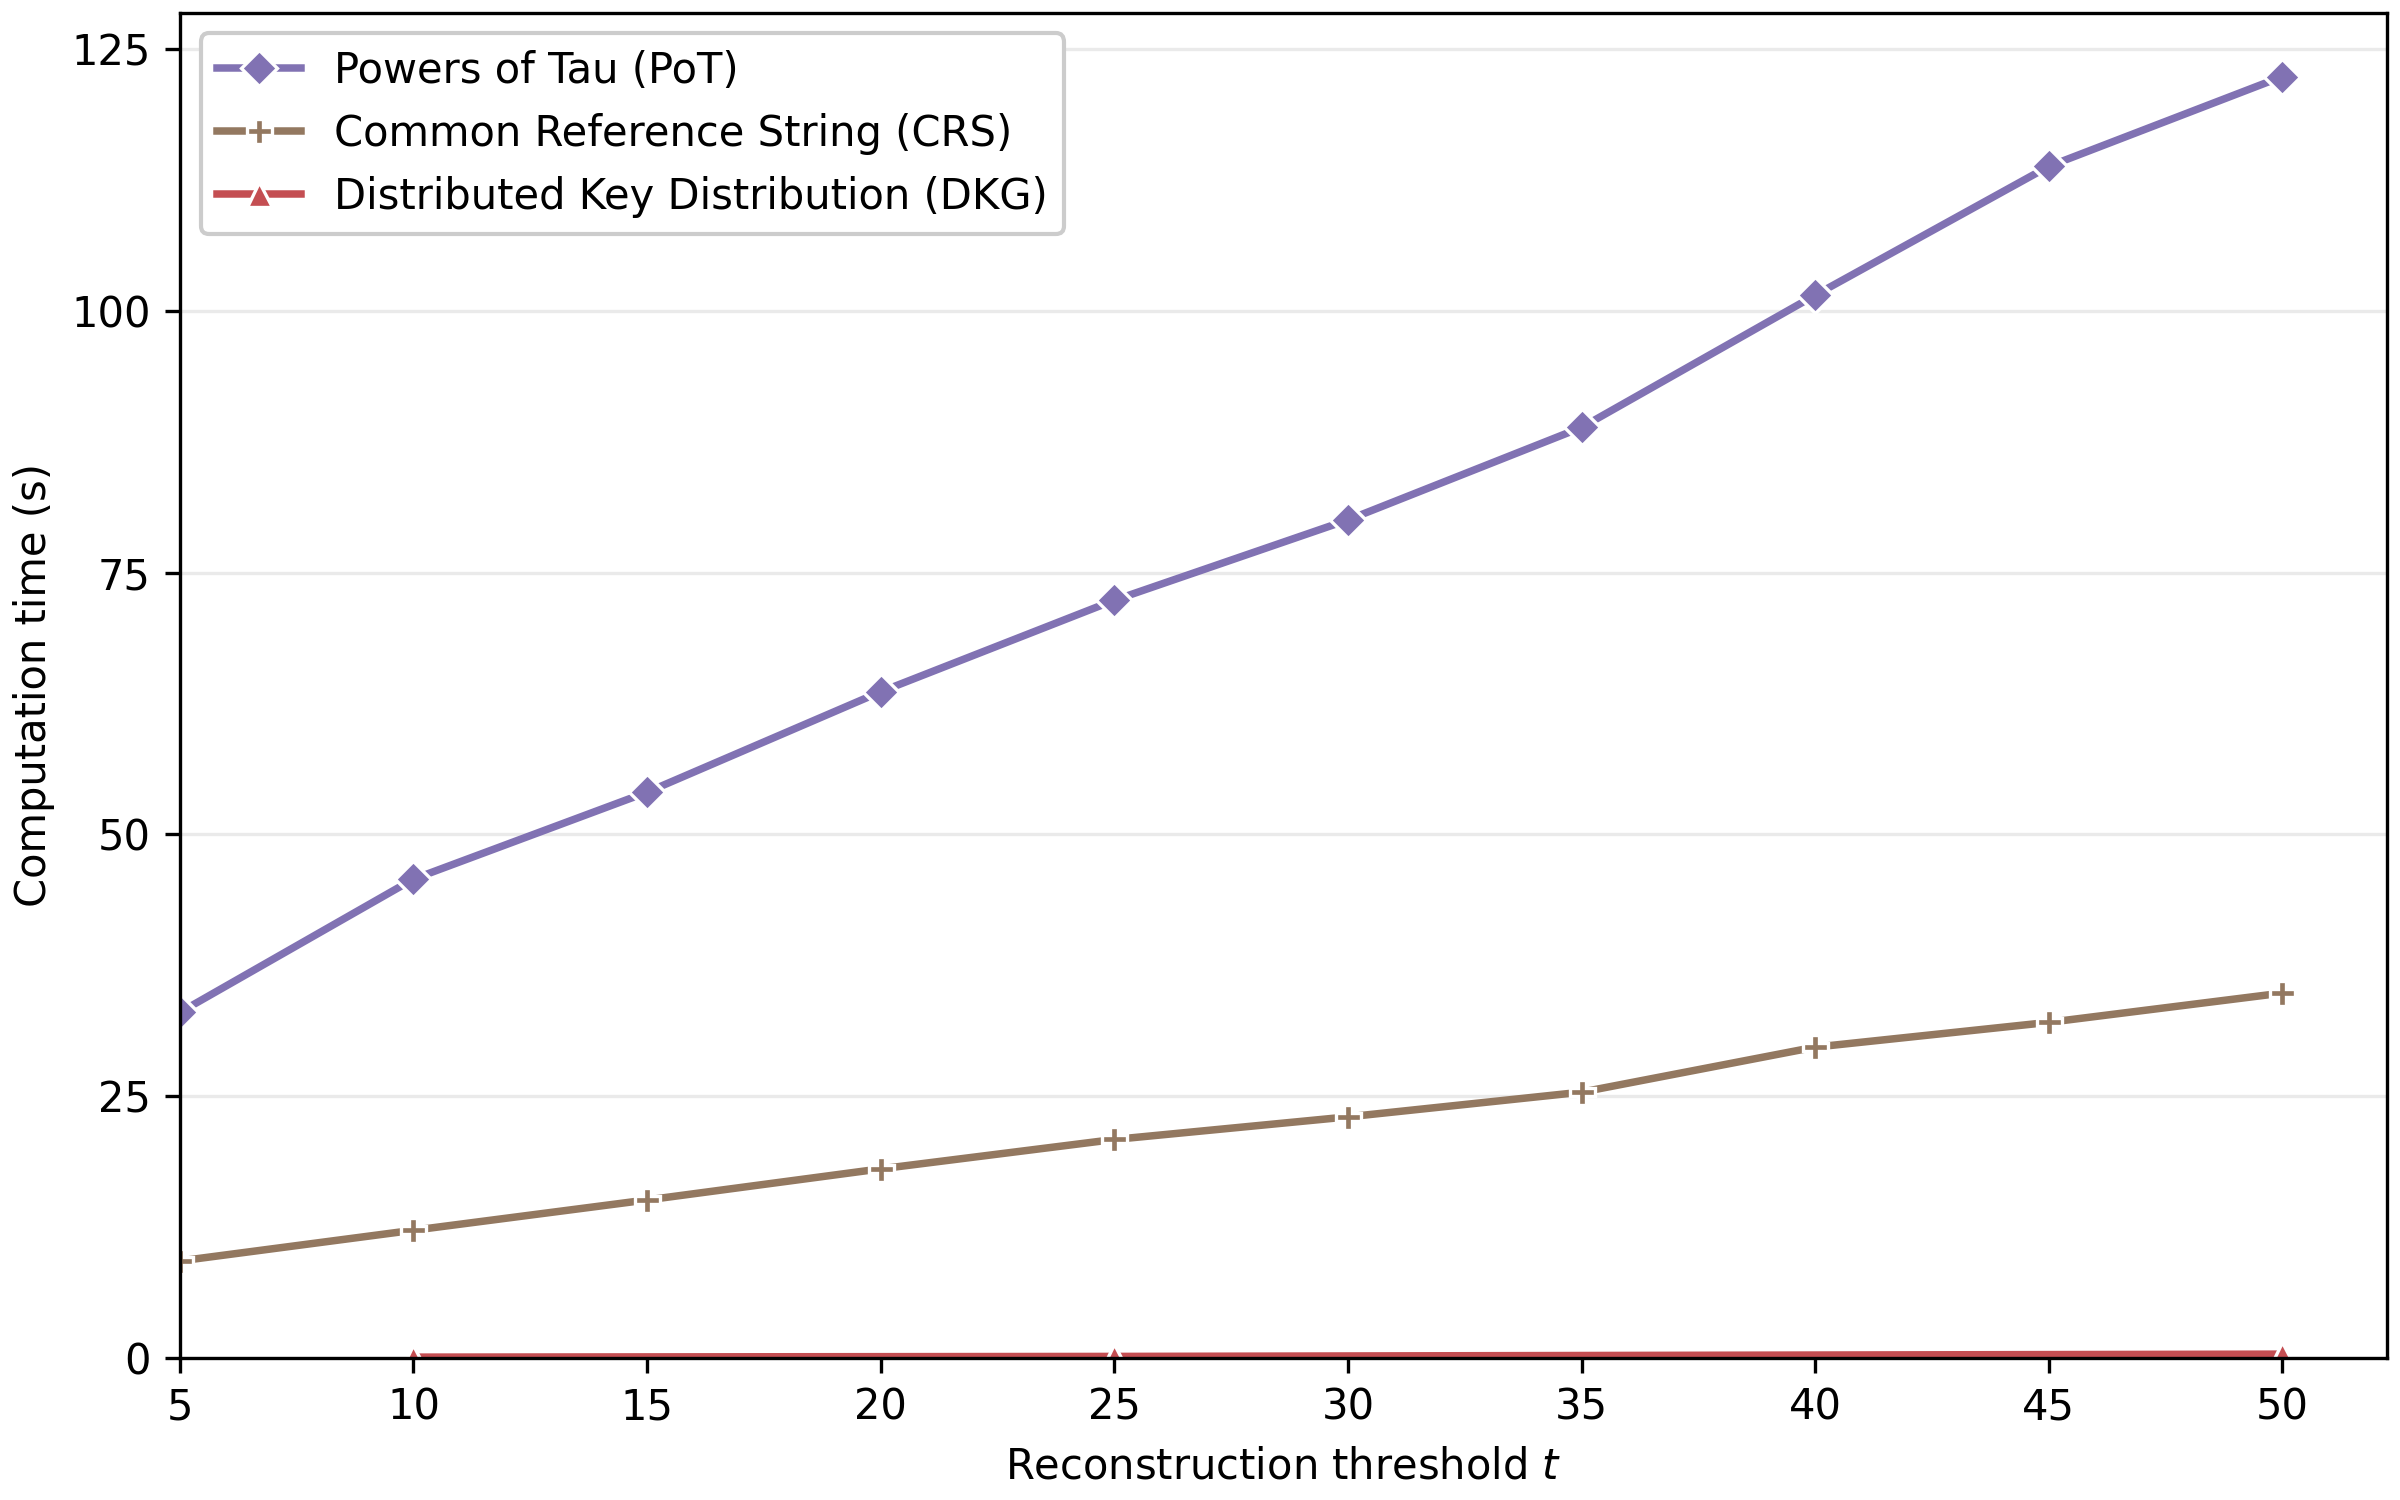
\includegraphics[width=\linewidth]{Images/setup.png}
    \caption{CPU time for DKG and ZK setup (PoT and CRS) as a function of the threshold $t$, where we consider $t$ contributions to each zero-knowledge setup phase.}
    \label{im:setup_time}
\end{figure}

\subsection{Credential issuance}

We separate credential issuance into client-side proof generation, proof verification by an authority, and the DSphinx specific credential-acquisition computation, including share aggregation.

For the fixed circuit, proof generation and verification is constant and require approximately $220\,\mathrm{ms}$ and $60\,\mathrm{ms}$ of CPU time, respectively. 
In the simulation, the client generates a proof once per run, while each participating authority verifies the proof when processing a credential request. 
The verification cost is therefore a per-authority measurement.

\todo[]{Rerun benchmark for credential issuance figure, the DSphinx cost of credential issuance as not been saved correctly...}
The DSphinx-specific computation increases with $t$, from approximately $40\,\mathrm{ms}$ at the smallest tested threshold to $200\,\mathrm{ms}$ at $t=50$ (Figure~\ref{im:credential_issuance}). 
This growth reflects the additional work required to aggregate authority shares using Lagrange interpolation. 
Proof generation is the most expensive operation in the credential issuance phase. 
\begin{figure}
    \centering
    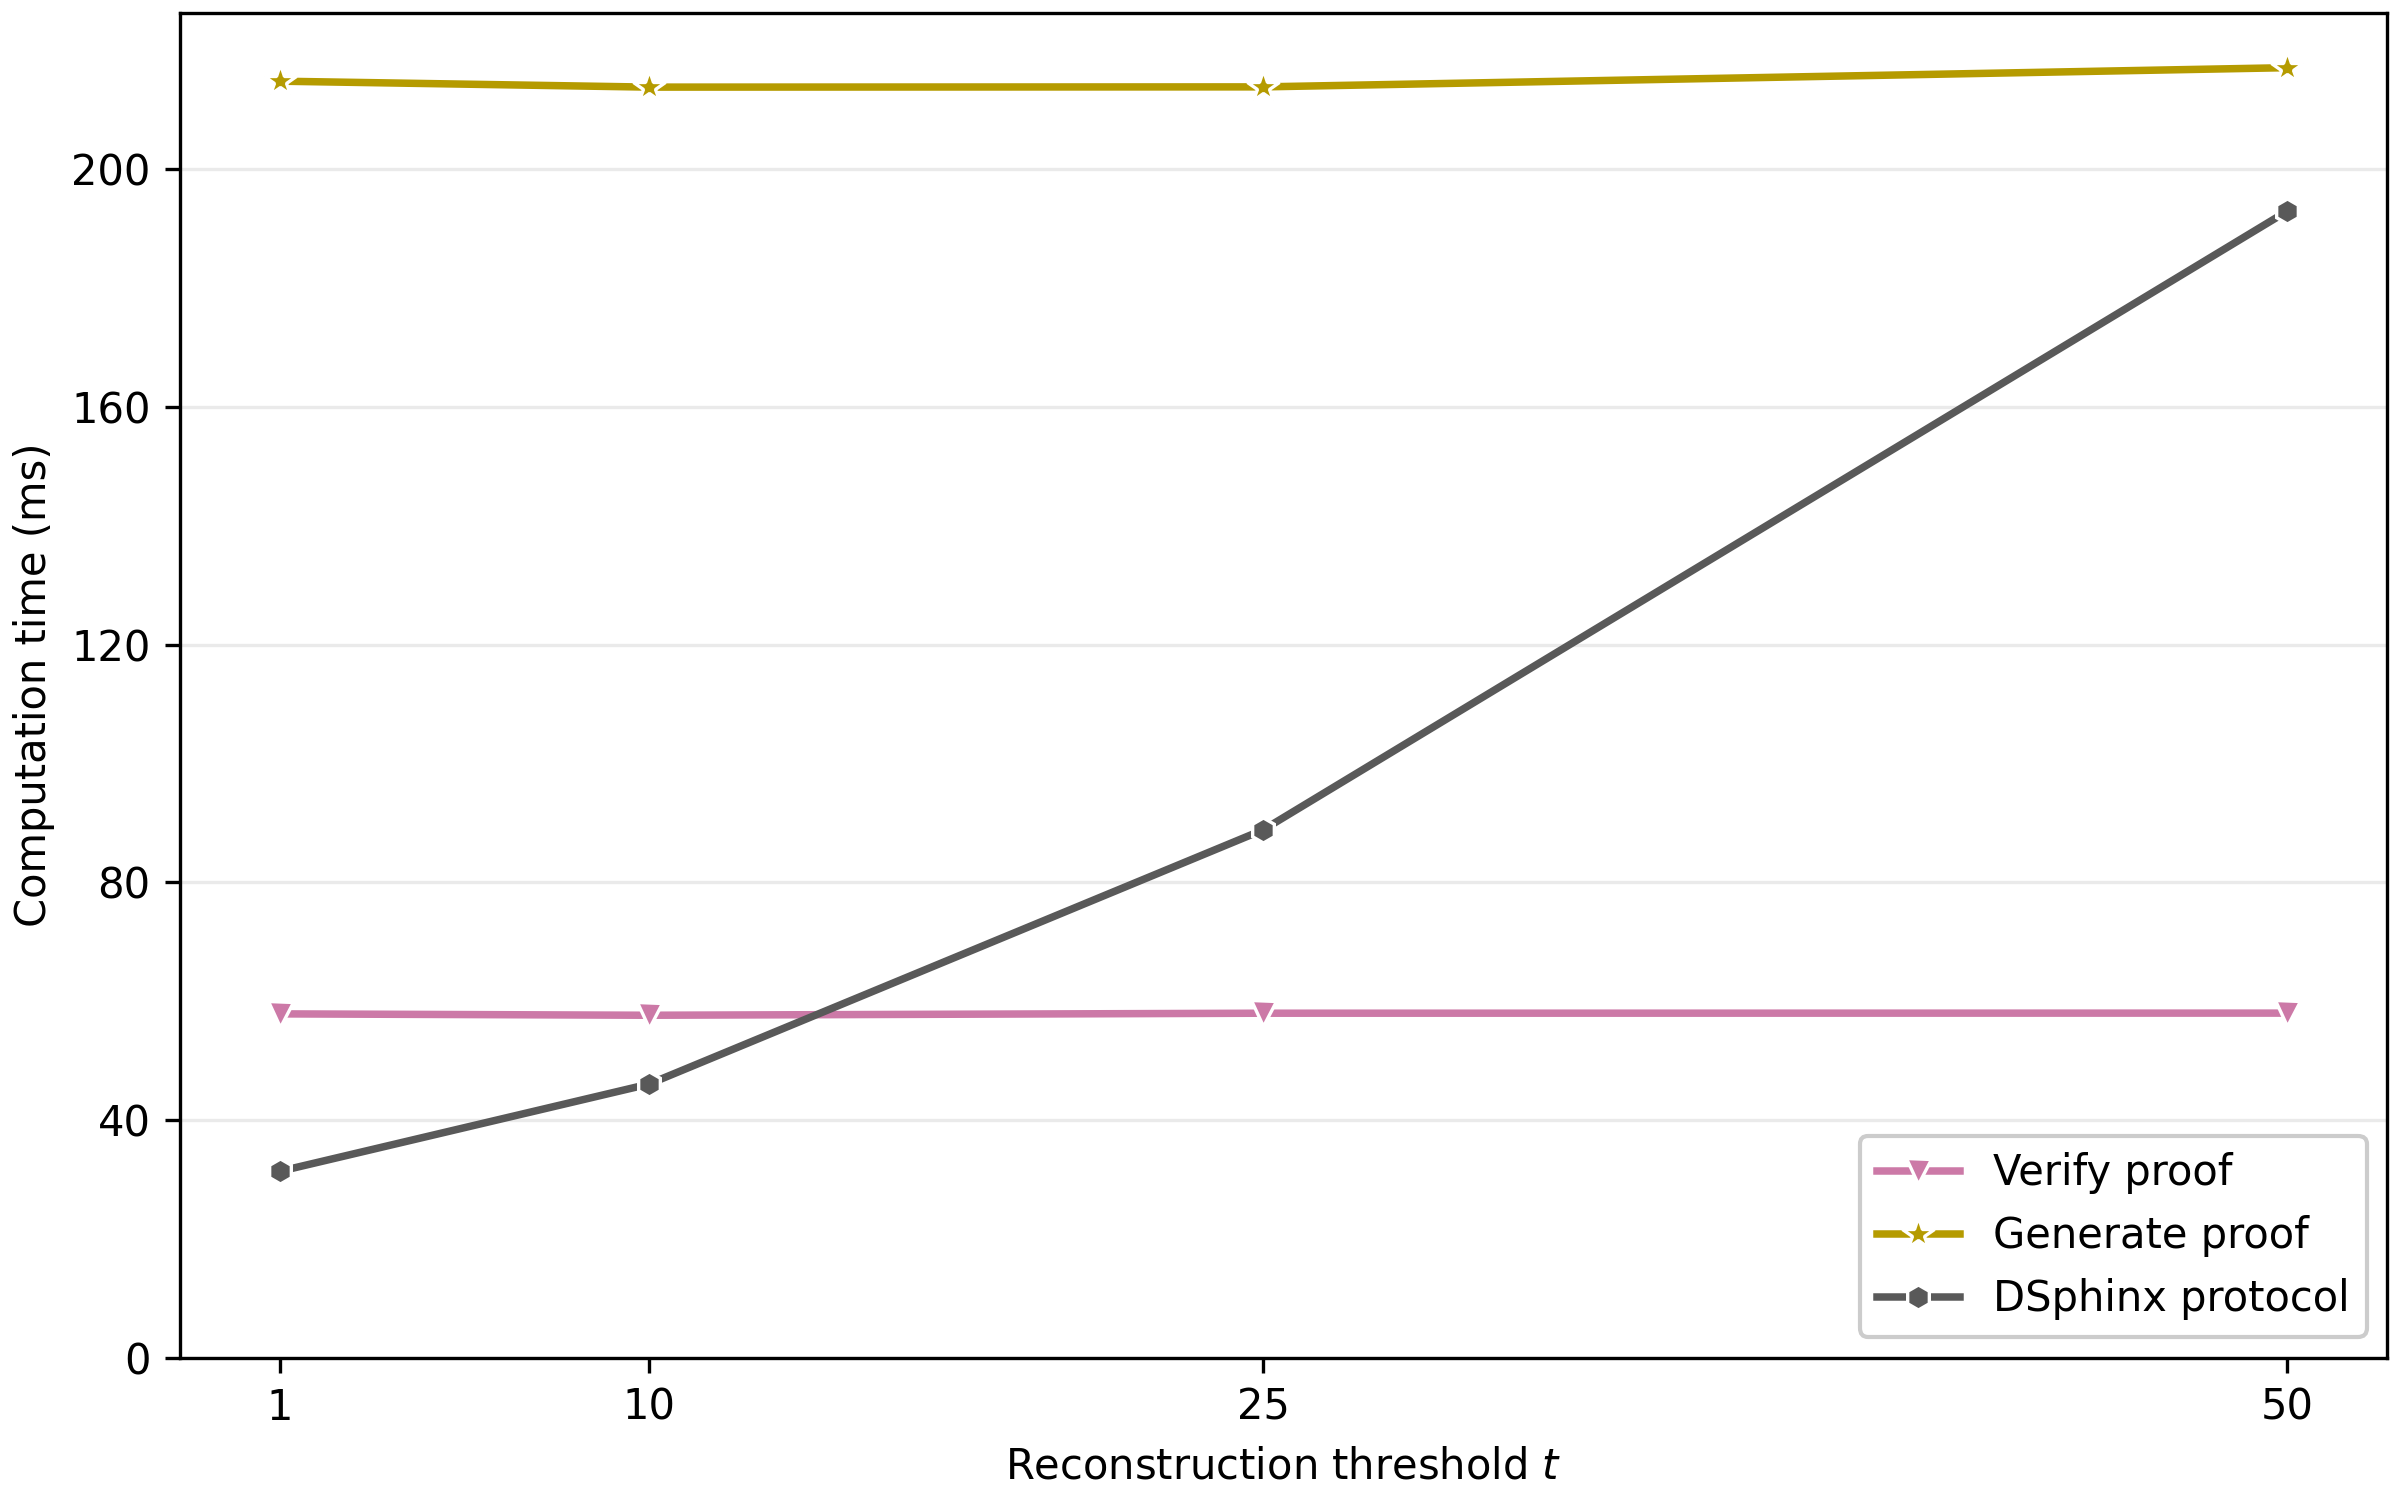
\includegraphics[width=\linewidth]{Images/credential_issuance.png}
    \caption{CPU time for client-side proof generation, proof verification at one authority, and DSphinx-specific credential-acquisition computation as a function of the reconstruction threshold $t$.}
    \label{im:credential_issuance}
\end{figure}

\subsection{Packet construction and processing}

We compare packet-header construction at the client (Figure~\ref{im:packet_time_client}) and per-packet processing at a mixnode (Figure~\ref{im:packet_time_mixnode}) for three configurations: 
Sphinx, DSphinx without credentials, and DSphinx with destination-bound credentials. 
We vary the path length $\ell$ from three to seven hops. 
The upper bound reflects the maximum path length supported by the Sphinx implementation used as our baseline. 

\todo[inline]{Need to rerun this part of the benchmark alone to remove the noise and have final result values...}
At the client, DSphinx requires approximately three times the CPU time of Sphinx for header construction. 
The measured cost nevertheless remains below $12\,\mathrm{ms}$ for a seven-hop path. 
Enabling credentials introduces a comparatively small additional cost, primarily associated with the credential-binding operation in Equation~\eqref{eq:header_bound_credential}.

At a mixnode, DSphinx adds approximately $1$ to $2\,\mathrm{ms}$ relative to Sphinx, and credential verification adds a further approximately $2\,\mathrm{ms}$. 
Although the additional cost is on the order of a few milliseconds per packet, it is substantial relative to the baseline since Sphinx processing remains approximately constant at $0.2\,\mathrm{ms}$ in these experiments. 
Credential-enabled processing therefore requires roughly an order of magnitude more computation than Sphinx. 
The two pairing operations in Equation~\eqref{eq:credential_verification} account for the dominant credential verification cost.

\begin{figure}
    \centering
    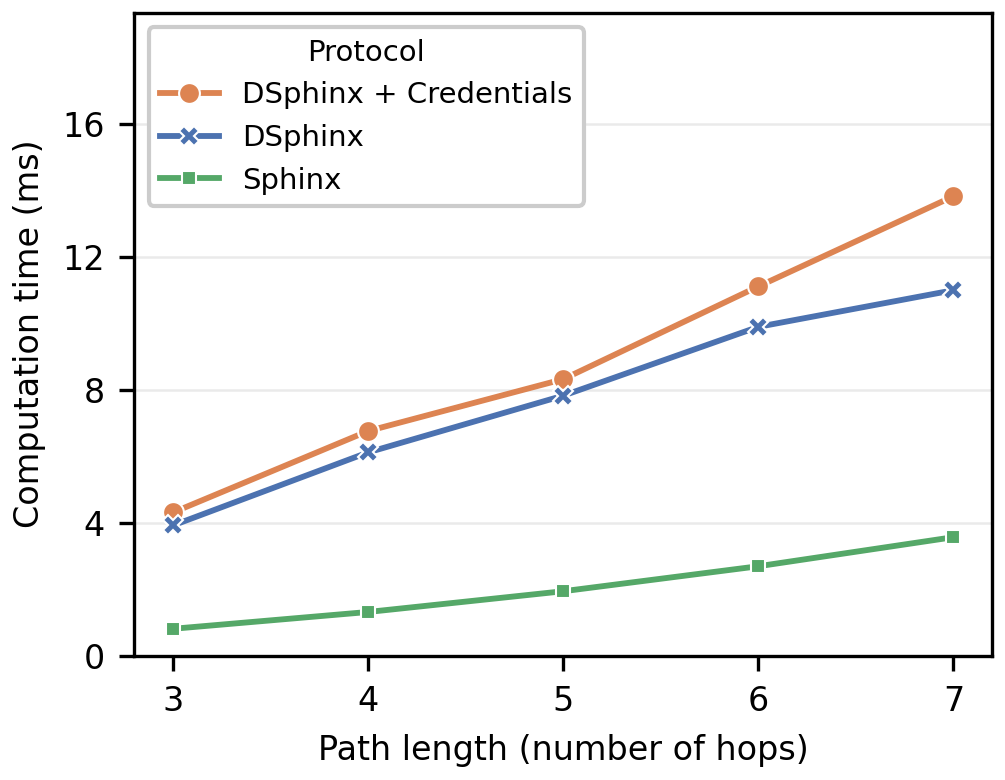
\includegraphics[width=\linewidth]{Images/packet_time_client.png}
    \caption{Mean CPU time for packet-header construction at the client as a function of the path length $\ell$, from three to seven hops.}
    \label{im:packet_time_client}
\end{figure}

\begin{figure}
    \centering
    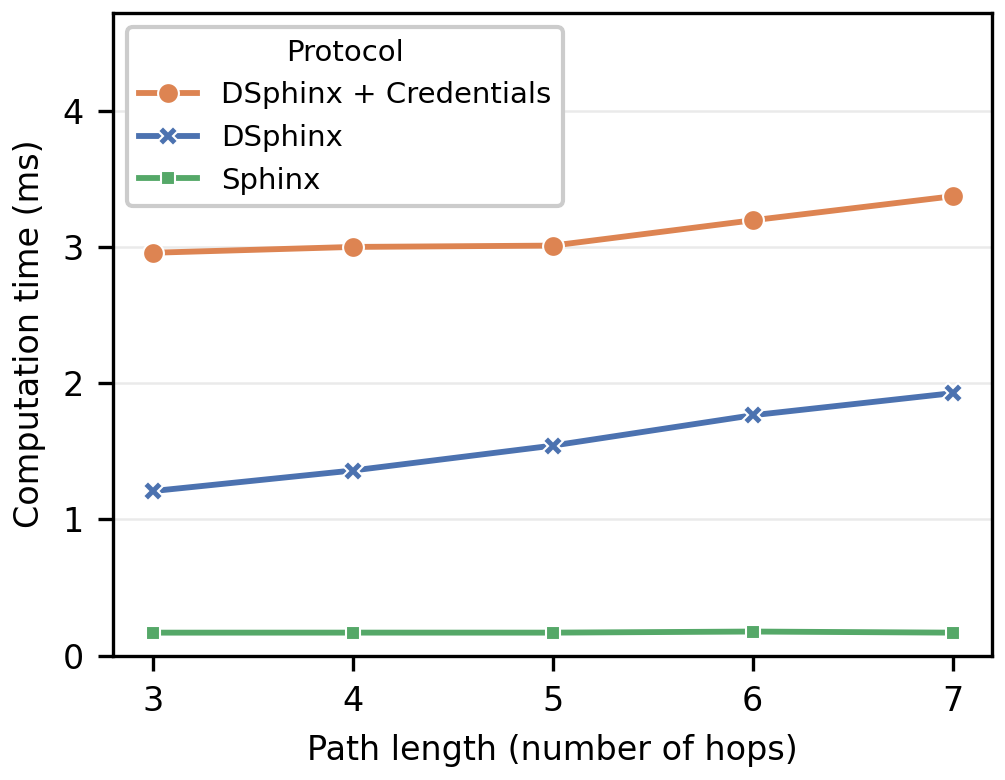
\includegraphics[width=\linewidth]{Images/packet_time_mixnode.png}
    \caption{Mean CPU time for processing one packet at a mixnode as a function of the path length $\ell$, from three to seven hops.}
    \label{im:packet_time_mixnode}
\end{figure}

%% DISUCSSION: Add 3-4 ms on mixnode but way cheaper than zk proof verification